\documentclass[10pt]{article}
\usepackage[margin=0.9in]{geometry}
\usepackage{newtxtext,newtxmath}
\usepackage{graphicx}
\usepackage{booktabs}
\usepackage{amsmath}
\usepackage[colorlinks=true,linkcolor=blue,citecolor=blue,urlcolor=blue]{hyperref}
\usepackage{caption}
\usepackage{float}
\captionsetup{font=small,labelfont=bf}
\graphicspath{{../figures/}}
\newcommand{\NoisyPthree}{14.60}
\newcommand{\NoisySthree}{0.054}
\newcommand{\NoisyFthree}{10.73}
\newcommand{\DenPthree}{30.31}
\newcommand{\DenSthree}{0.835}
\newcommand{\DenFthree}{23.80}
\newcommand{\DecPthree}{31.34}
\newcommand{\DecSthree}{0.885}
\newcommand{\DecFthree}{24.61}
\newcommand{\UNetPthree}{32.27}
\newcommand{\UNetSthree}{0.907}
\newcommand{\UNetFthree}{25.25}
\newcommand{\NoisyPten}{19.53}
\newcommand{\NoisySten}{0.151}
\newcommand{\NoisyFten}{15.25}
\newcommand{\DenPten}{32.50}
\newcommand{\DenSten}{0.905}
\newcommand{\DenFten}{25.33}
\newcommand{\DecPten}{33.62}
\newcommand{\DecSten}{0.917}
\newcommand{\DecFten}{26.77}
\newcommand{\UNetPten}{34.74}
\newcommand{\UNetSten}{0.934}
\newcommand{\UNetFten}{27.68}
\newcommand{\NoisyPthirty}{24.10}
\newcommand{\NoisySthirty}{0.331}
\newcommand{\NoisyFthirty}{19.60}
\newcommand{\DenPthirty}{34.08}
\newcommand{\DenSthirty}{0.923}
\newcommand{\DenFthirty}{26.91}
\newcommand{\DecPthirty}{35.34}
\newcommand{\DecSthirty}{0.937}
\newcommand{\DecFthirty}{28.39}
\newcommand{\UNetPthirty}{36.70}
\newcommand{\UNetSthirty}{0.950}
\newcommand{\UNetFthirty}{29.67}
\newcommand{\NoisyPonehundred}{28.81}
\newcommand{\NoisySonehundred}{0.596}
\newcommand{\NoisyFonehundred}{23.92}
\newcommand{\DenPonehundred}{35.36}
\newcommand{\DenSonehundred}{0.935}
\newcommand{\DenFonehundred}{28.22}
\newcommand{\DecPonehundred}{37.16}
\newcommand{\DecSonehundred}{0.952}
\newcommand{\DecFonehundred}{30.22}
\newcommand{\UNetPonehundred}{38.61}
\newcommand{\UNetSonehundred}{0.963}
\newcommand{\UNetFonehundred}{31.63}
\newcommand{\NoisyPthreehundred}{32.48}
\newcommand{\NoisySthreehundred}{0.793}
\newcommand{\NoisyFthreehundred}{26.95}
\newcommand{\DenPthreehundred}{36.26}
\newcommand{\DenSthreehundred}{0.947}
\newcommand{\DenFthreehundred}{29.01}
\newcommand{\DecPthreehundred}{38.63}
\newcommand{\DecSthreehundred}{0.963}
\newcommand{\DecFthreehundred}{31.67}
\newcommand{\UNetPthreehundred}{40.01}
\newcommand{\UNetSthreehundred}{0.971}
\newcommand{\UNetFthreehundred}{33.03}
\newcommand{\DecGainThree}{0.93}
\newcommand{\DecCIThree}{0.83--1.05}
\newcommand{\DecGainTen}{1.12}
\newcommand{\DecCITen}{1.06--1.19}
\newcommand{\DecGainThirty}{1.36}
\newcommand{\DecCIThirty}{1.23--1.49}
\newcommand{\DecGainHundred}{1.45}
\newcommand{\DecCIHundred}{1.34--1.57}
\newcommand{\DecGainThreeHundred}{1.37}
\newcommand{\DecCIThreeHundred}{1.25--1.51}
\newcommand{\DenGainThree}{1.96}
\newcommand{\BestGainThree}{0.93}
\newcommand{\BestGainThirty}{1.36}
\newcommand{\BestGainThreeHundred}{1.37}
\newcommand{\BestGainMin}{0.93}
\newcommand{\BestGainMax}{1.45}
\newcommand{\PSNRThirtyTwoDec}{30}
\newcommand{\PSNRThirtyTwoU}{10}
\newcommand{\PSNRThirtyTwoFactor}{3.0}
\newcommand{\SSIMNineDec}{30}
\newcommand{\SSIMNineU}{10}
\newcommand{\SSIMNineFactor}{3.0}
\newcommand{\SSIMNineTwoDec}{30}
\newcommand{\SSIMNineTwoU}{30}
\newcommand{\SSIMNineTwoFactor}{1.0}
\newcommand{\FGTwoSixDec}{100}
\newcommand{\FGTwoSixU}{30}
\newcommand{\FGTwoSixFactor}{3.3}
\newcommand{\CrossDecFourteen}{1.36}
\newcommand{\CrossDecFifteen}{0.52}
\newcommand{\CrossDecSixteen}{1.30}
\newcommand{\CrossDecEighteen}{0.16}
\newcommand{\CrossDecMin}{0.16}
\newcommand{\CrossDecMax}{1.30}
\newcommand{\SpecPthree}{32.36}
\newcommand{\SpecSthree}{0.908}
\newcommand{\SpecFthree}{25.32}
\newcommand{\SpecPthirty}{36.72}
\newcommand{\SpecSthirty}{0.951}
\newcommand{\SpecFthirty}{29.67}
\newcommand{\SpecPonehundred}{38.68}
\newcommand{\SpecSonehundred}{0.963}
\newcommand{\SpecFonehundred}{31.74}
\newcommand{\CondPthree}{32.20}
\newcommand{\CondSthree}{0.905}
\newcommand{\CondFthree}{25.17}
\newcommand{\CondPthirty}{36.44}
\newcommand{\CondSthirty}{0.948}
\newcommand{\CondFthirty}{29.34}
\newcommand{\CondPonehundred}{38.29}
\newcommand{\CondSonehundred}{0.961}
\newcommand{\CondFonehundred}{31.27}
\newcommand{\BlindPthree}{32.27}
\newcommand{\BlindSthree}{0.907}
\newcommand{\BlindFthree}{25.25}
\newcommand{\ScrPthree}{30.19}
\newcommand{\BlindPthirty}{36.70}
\newcommand{\BlindSthirty}{0.950}
\newcommand{\BlindFthirty}{29.67}
\newcommand{\ScrPthirty}{34.46}
\newcommand{\BlindPonehundred}{38.61}
\newcommand{\BlindSonehundred}{0.963}
\newcommand{\BlindFonehundred}{31.63}
\newcommand{\ScrPonehundred}{36.18}
\newcommand{\CondDeltaLow}{-0.33}
\newcommand{\CondDeltaHigh}{-0.07}
\newcommand{\CondStrongPthree}{32.29}
\newcommand{\CondStrongPthirty}{36.71}
\newcommand{\CondStrongPonehundred}{38.66}
\newcommand{\CondStrongLow}{+0.01}
\newcommand{\CondStrongHigh}{+0.05}
\newcommand{\CondStrongDelta}{0.05}
\newcommand{\AucThree}{0.96}
\newcommand{\AucTen}{0.96}
\newcommand{\NFailThirty}{1}
\newcommand{\RhoThree}{0.92}
\newcommand{\SigmaUPfifteen}{36.92}
\newcommand{\SigmaDecfifteen}{35.85}
\newcommand{\SigmaUPtwo}{36.70}
\newcommand{\SigmaDectwo}{35.34}
\newcommand{\SigmaUPtwopfive}{35.76}
\newcommand{\SigmaDectwopfive}{34.76}
\newcommand{\AiryStrongUThree}{32.63}
\newcommand{\AiryStrongGainThree}{+1.42}
\newcommand{\AiryStrongUThirty}{36.64}
\newcommand{\AiryStrongGainThirty}{+0.41}
\newcommand{\AiryStrongUThreeHundred}{37.05}
\newcommand{\AiryStrongGainThreeHundred}{-3.21}
\newcommand{\AiryUThree}{32.71}
\newcommand{\AiryTvThree}{31.21}
\newcommand{\AiryGainThree}{1.50}
\newcommand{\AiryCIThree}{1.35--1.65}
\newcommand{\AiryUThirty}{37.61}
\newcommand{\AiryTvThirty}{36.23}
\newcommand{\AiryGainThirty}{1.39}
\newcommand{\AiryCIThirty}{1.28--1.48}
\newcommand{\AiryUThreeHundred}{41.55}
\newcommand{\AiryTvThreeHundred}{40.26}
\newcommand{\AiryGainThreeHundred}{1.29}
\newcommand{\AiryCIThreeHundred}{1.13--1.45}
\newcommand{\PsfMixGaussPThree}{32.26}
\newcommand{\PsfMixGaussPThirty}{36.60}
\newcommand{\PsfMixGaussPThreeHundred}{39.83}
\newcommand{\HeldoutPFive}{33.32}
\newcommand{\HeldoutPFifty}{37.50}
\newcommand{\HeldoutPTwoHundred}{39.47}
\newcommand{\HeldoutResFive}{0.00}
\newcommand{\HeldoutResFifty}{0.01}
\newcommand{\HeldoutResTwoHundred}{0.02}
\newcommand{\SpeedCPU}{29.3}
\newcommand{\SpeedGPU}{1.2}
\newcommand{\SpeedTV}{103}
\newcommand{\SpeedFactorCPU}{3.5}
\newcommand{\SpeedFactorGPU}{86}

\newcommand{\RealN}{243}
\newcommand{\RealNoisyP}{16.44}
\newcommand{\RealNoisyS}{0.107}
\newcommand{\RealBMThreeP}{24.83}
\newcommand{\RealBMThreeS}{0.559}
\newcommand{\RealNlmP}{24.78}
\newcommand{\RealNlmS}{0.551}
\newcommand{\RealTvP}{24.51}
\newcommand{\RealTvS}{0.526}
\newcommand{\RealUnetP}{29.01}
\newcommand{\RealUnetS}{0.877}
\newcommand{\RealBMThreeRawP}{21.30}
\newcommand{\RealBMThreeRawS}{0.359}
\newcommand{\RealNlmRawP}{21.28}
\newcommand{\RealNlmRawS}{0.354}
\newcommand{\RealTvRawP}{20.58}
\newcommand{\RealTvRawS}{0.333}
\newcommand{\RealGain}{4.18}
\newcommand{\RealGainRaw}{7.70}
\newcommand{\RealCI}{3.94--4.42}
\newcommand{\RealGainNlm}{4.23}
\newcommand{\RealGainTv}{4.50}
\newcommand{\RealWins}{240}
\newcommand{\RealPvalue}{2.2e-41}
\newcommand{\RealBmSigma}{0.3}
\newcommand{\RealNlmH}{0.2}
\newcommand{\RealTvW}{0.24}
\newcommand{\RealDncnnP}{28.80}
\newcommand{\RealDncnnS}{0.865}
\newcommand{\RealDncnnGain}{3.97}
\newcommand{\RealUnetGainDncnn}{0.21}
\newcommand{\RealUnetDncnnCI}{0.15--0.28}
\newcommand{\RealUnetDncnnWins}{210}
\newcommand{\LargeRealN}{20}
\newcommand{\LargeRealNoisyP}{13.35}
\newcommand{\LargeRealBMThreeP}{17.05}
\newcommand{\LargeRealNlmP}{16.89}
\newcommand{\LargeRealTvP}{16.45}
\newcommand{\LargeRealUnetP}{15.83}

\newcommand{\FmdN}{150}
\newcommand{\FmdNoisyP}{25.62}
\newcommand{\FmdNoisyS}{0.584}
\newcommand{\FmdBMThreeP}{28.07}
\newcommand{\FmdBMThreeS}{0.704}
\newcommand{\FmdNlmP}{26.96}
\newcommand{\FmdNlmS}{0.697}
\newcommand{\FmdTvP}{27.01}
\newcommand{\FmdTvS}{0.707}
\newcommand{\FmdUnetP}{31.74}
\newcommand{\FmdUnetS}{0.845}
\newcommand{\FmdGain}{3.67}
\newcommand{\FmdWins}{147}
\newcommand{\FmdPvalue}{2.9e-26}
\newcommand{\FmdCI}{3.27--4.12}
\newcommand{\FmdStrataMin}{0.4}
\newcommand{\FmdStrataMax}{11.1}
\newcommand{\FmdStrataN}{36}

\title{\bfseries Dose-agnostic neural deconvolution for\\
low-dose fluorescence microscopy}
\author{}
\date{\today}
\begin{document}
\maketitle

\begin{abstract}
Fluorescence microscopy is photon-limited: the light that improves
signal-to-noise also drives photobleaching and phototoxicity. Computational
restoration can recover structure from fewer photons, but the regularization
that works at one noise level fails at another, and most learned models are
trained or conditioned for a narrow dose range. In practice the photon count is
often unknown, varies across the field, and changes with acquisition settings,
so per-dose retuning is difficult to deploy. Here we ask whether a single model
can cover a wide dose range without dose metadata, and how much photon budget
that saves against a well-tuned classical method.

We train one U-Net on mixed-dose patches with no photon-count input and compare
it with TV-ADMM deconvolution tuned at every dose across a 100-fold range. To
make the comparison operational, we select the dose on validation fields for a
target success rate and apply it unchanged to held-out fields. The same model
improves over tuned TV-ADMM by \BestGainMin--\BestGainMax\,dB across the range,
needs a 3--3.3$\times$ lower photon budget at matched 90\% success on several
criteria, and, on real noisy/clean pairs (a denoising check), improves over
affine-calibrated BM3D by \RealGain\,dB. Controls show that this gain comes
from learned sample structure rather than capacity, and a PSF-mixed variant
retains it under an Airy PSF. The dose sweep is simulated and the real gain is
in-source; together they show that one model can replace per-dose tuning and
that restoration methods should be compared at matched success rather than at a
single dose.
\end{abstract}

\section{Introduction}
Fluorescence microscopy is limited by the number of detected photons. Raising
excitation power or exposure improves signal-to-noise ratio, but it also
accelerates photobleaching and phototoxicity, which is especially restrictive
for live samples \cite{laissue2017phototoxicity}. Computational restoration
offers a way out: recover more of the underlying structure from the photons
already collected. Deconvolution removes the diffraction-limited point-spread
function (PSF) while suppressing shot noise, but the inverse problem becomes
increasingly ill-posed as the photon count falls. A regularization strength
that preserves fine structure at one dose amplifies noise at a lower dose; one
that suppresses noise at low dose erases structure at a higher dose.

Classical deconvolution makes this trade-off explicit. Richardson--Lucy
\cite{richardson1972,lucy1974}, Wiener filtering \cite{wiener1949}, total
variation \cite{chambolle2004,rudin1992}, non-local means \cite{buades2005},
and blind deconvolution \cite{kundur1996} all depend on a noise model and a
regularization weight that must be chosen for a particular signal level; see
Ref.~\cite{wallace2001} for a review. Deep learning replaces the hand-designed
prior with one learned from paired images. CARE \cite{weigert2018care} and its
deployment tools \cite{gomez2021deepimagej} have made U-Net restoration
routine, and supervised restoration has been extended to cross-modality
super-resolution \cite{wang2019crossmodality}. Noise-level conditioning is
standard in image denoising \cite{zhang2018ffdnet}, and blind denoisers can
estimate it or learn without an explicit noise level
\cite{guo2019cbdnet,mohan2020biasfree,krull2019}, but these methods denoise
rather than deconvolve and have not been evaluated at a matched success rate
across a wide dose range. Model-based deep deconvolution
\cite{liu2020degeneration}, zero-shot deconvolution from noisy images alone
\cite{qiao2024zsdeconvnet}, uncertainty-guided adaptive scanning
\cite{ye2025uncertainty}, and near-zero-photon imaging
\cite{sheneman2025nearzero} address complementary parts of the problem. In
microscopy, however, the photon count per pixel is often not known precisely,
varies across the field, and changes with acquisition settings. Retuning or
retraining for every dose is practical only within a narrow range. The
practical question for low-dose imaging is whether one model can cover a wide
dose range without being told the dose, and how much photon budget that saves
against a well-tuned classical method. The contribution is not a new network
architecture; it is a controlled test of that question, with the saving
measured at matched success rather than at a single dose.

We address this with a controlled study on public microscopy images. One U-Net
is trained on patches whose dose is sampled over a 100-fold range; the network
receives only the noisy image and has no dose channel, so it must infer the
local noise level from the data. We compare against total-variation (TV)
deconvolution with the known PSF, TV denoising, Wiener filtering, and
Richardson--Lucy, all tuned per dose; NLM denoising is included in the
qualitative and extended comparisons. Splits are by field of view (FOV), and
test FOVs are never used for training, tuning, or early stopping. To make the
comparison operational, we define a protocol criterion: choose the smallest
dose that reaches 90\% success on validation FOVs, then apply it unchanged to
held-out FOVs. This avoids selecting the operating point on the test data and
turns the dose-response curves into a photon-budget comparison.

Across this range, the blind model improves over tuned TV-ADMM by
\BestGainMin--\BestGainMax\,dB at every dose and needs a 3--3.3$\times$ lower
photon budget at matched 90\% success on several criteria. It also transfers to
three held-out stains with smaller positive gains. The real-data check tests
denoising: with retraining on the same acquisition protocol, the network
improves over affine-calibrated BM3D by \RealGain\,dB, while a budget-matched
DnCNN is close behind. Controls separate the source of the gain: a
budget-matched phase-scrambled network falls below TV, whereas dose
conditioning and per-dose specialists add little, so the gain is not explained
by capacity or metadata. A PSF-mixed variant keeps the gain under a physical Airy PSF,
where the Gaussian-trained model loses its high-dose advantage (SI S4d).

Practically, this removes one calibration axis. In live imaging the acceptable
dose is set by the sample rather than by the restoration algorithm; a model
that covers the full range without metadata can be trained once and reused as
the protocol changes, and the protocol curve selects the dose that reaches a
desired quality. It also changes how restoration methods should be compared: a
gain measured at one dose can shrink or grow at another, so the meaningful
quantity is the photon budget required at a matched success rate. The scope is limited in two ways: the dose sweep is simulated with a
known Gaussian PSF and Poisson noise, and the real pairs test restoration
within one acquisition protocol; the same weights do not transfer zero-shot to
a different source. Within that scope, the results support dose-agnostic
restoration.

\section{Methods}
\paragraph{Forward model.}
A clean FOV $x$ is blurred by a Gaussian PSF of width $\sigma$ and corrupted by
Poisson shot noise,
\begin{equation}
y = \frac{1}{P}\operatorname{Poisson}\!\left(P\,(g_\sigma * x)\right),
\label{eq:forward}
\end{equation}
where $P$ is a full-scale Poisson scale: a pixel with normalized intensity $x$
has expected detected photons $Px$. Unless stated otherwise $\sigma=2$ pixels
and $P$ ranges from 3 to 300 in full-scale units. The same PSF is used to generate the
data and by all classical baselines. For brevity we call $P$ the dose; the
mean detected photons per pixel on the test patches are 0.36, 3.56, and 35.6
at $P=3,30,300$, respectively (Poisson means in
\texttt{results/photon\_units.json}). Because the expected count scales
linearly with $P$, a ratio in $P$ is also a ratio in photon budget.

\paragraph{Data.}
We use four public datasets from the Broad Bioimage Benchmark Collection
\cite{ljosa2012bbbc}. The main dataset is BBBC014 channel~1 (96 FOVs,
$1360\times1024$ pixels, 8-bit, CC~BY~3.0), split at the FOV level into 56
training, 20 validation, and 20 test FOVs. Validation FOVs are used for early
stopping and for tuning every classical baseline; test FOVs are never used for
training, tuning, or model selection. BBBC015 and BBBC016 (U2OS
cytoplasm-to-nucleus assays; CC~BY~3.0) and BBBC018 (actin channel; a different
cell type and stain; CC~BY-NC-SA~3.0) are used only as external test sets, with
20 FOVs sampled uniformly from each (five for TV tuning and 15 held out for evaluation). All images are normalized by their 8-bit full scale.

\paragraph{Real noisy/clean data.}
For a real-noise check we use the public AI4Life-MDC25-Nuclei release
\cite{ai4life_mdc25_2025} (Zenodo 15624741, CC~BY~4.0), the training set of the
2025 AI4Life Microscopy Supervised Denoising Challenge. It combines 2{,}457
$256\times256$ pairs from the Jacquemet noisy-nuclei source with 20
$1024\times1024$ pairs from BBBC006; the two sources differ in bit depth,
saturation, and noise model. We exclude the 20 small-pair IDs that coincide
numerically with the large-field IDs as a precaution (the images are not crops
of one another), leaving 2{,}437 pairs split by image ID into 1{,}951 training,
243 validation, and 243 test pairs. No field is shared: over all 1{,}951
training images, the maximum test-train thumbnail correlation is 0.55, no pair
exceeds 0.8, and the top pair has full-resolution correlation 0.06
(\texttt{results/real\_leakage\_full.json}). The
real-data comparison uses all \RealN\ held-out pairs; classical outputs are
affine-calibrated on the validation pairs (Methods, Real-data model). The 20
large BBBC006 pairs are never used for training
or tuning and form a cross-source transfer check.

\paragraph{Second real source.}
The FMD release \cite{zhang2019fmd,ai4life_mdc25_fmd_2025} (Zenodo 15761900, CC~BY~4.0)
contains 63{,}669 $256\times256$ noisy/clean pairs (multiple frames per field)
from three microscopes, three channels, and four noise levels. We use one frame
from each of 1{,}998 fields (seed 0) and split by field, stratified by
microscope/channel/level, into 1{,}396/301/301
training/validation/test; no frame of a field crosses splits. The main
comparison uses a pre-specified 150-field subset: the first four fields per
stratum in field-ID order, plus six fifth fields, selected before prediction.

\paragraph{Network and training.}
The network is a three-level U-Net \cite{ronneberger2015unet} with 64, 128, and
256 channels and $3\times3$ convolutions. Training patches are $64\times64$
pixels drawn from training FOVs, with random flips and $90^\circ$ rotations.
The main mixed-dose model samples the dose of every patch from
$\{3,10,30,100,300\}$ full-scale units and receives only the noisy image; no
dose channel is used at training or inference. It uses 48{,}000 patches and a
150-epoch schedule with early stopping on validation PSNR averaged over all
doses. A PSF-robust variant uses the same schedule but randomly blurs each
training patch with the Gaussian ($\sigma=2$) or a scalar Airy PSF (NA 1.4,
$\lambda=520$\,nm, 100\,nm pixels). Optimization
uses Adam with a learning rate of $10^{-3}$, a cosine schedule, and a
mean-squared-error loss. A base-budget ablation uses a 32-channel
conditioned variant (24{,}000 patches, 100 epochs); a budget-matched
conditioned model repeats the full 64-channel/48{,}000-patch/150-epoch
schedule. The conditioned variant adds a constant dose channel
$c(P)=(\log_{10}P-\log_{10}3)/(\log_{10}300-\log_{10}3)$. Per-dose specialists
use the same 64-channel/48{,}000-patch/150-epoch schedule, trained at 3, 30, or
100 full-scale units. Two phase-scrambled controls replace every training FOV by a
random-phase surrogate with the same power spectrum while keeping validation
and test FOVs unchanged: a base-budget control (32 channels, 24{,}000 patches,
100 epochs) and a budget-matched blind control (64 channels, 48{,}000 patches,
150 epochs, mixed doses). Validation uses four spread $128\times128$ patches
per FOV.

\paragraph{Real-data model.}
The real-data network is a CARE-style supervised U-Net (the same three-level
encoder--decoder used for the simulation model, with 48 channels in the first
level) and is trained on $128\times128$ patches from the real training pairs
(16{,}000 patches, 80 epochs, batch 64, Adam with learning rate $10^{-3}$,
cosine schedule), with flips and $90^\circ$ rotations. Each image is normalized
independently to its 0.5--99.9 percentile range. Validation on the 243 held-out
small pairs selects the checkpoint (28.6\,dB). For the nuclei pairs, classical baselines are tuned
on five validation pairs over extended grids (BM3D \cite{dabov2007}
$\sigma\in[0.2,1.0]$, NLM
$h\in[0.1,0.3]$, TV weight $\in[0.08,0.4]$); the selected values are
$\sigma=\RealBmSigma$, $h=\RealNlmH$, and $w=\RealTvW$ (grid means in
\texttt{results/real\_small\_tuning\_grid.json}). Each classical output is
additionally mapped by one global affine transform (gain and offset) fitted on
the validation pairs, because the supervised networks are trained on paired
images; raw uncalibrated values are in the SI. A second supervised baseline
is a 17-layer DnCNN \cite{zhang2017dncnn} with 64 channels and residual noise
prediction, trained on 16{,}000 patches for 80 epochs with the same
normalization and augmentation (validation 28.2\,dB). The FMD model uses the smaller base budget (32
channels, 8{,}000 patches, 40 epochs) and is therefore a secondary check.
Its classical baselines are tuned separately for each microscope on five
validation fields: the selected BM3D sigmas are 0.12 (CF), 0.15 (TP), and 8.0
(WF), where the WF search was extended to 20 to avoid a boundary solution; NLM
uses $h=0.1$, and TV weights are 0.08 (CF) and 0.12 (TP, WF). The FMD
checkpoint is selected on 60 FMD validation fields. Test pairs are never used
for tuning or early stopping.

\paragraph{Baselines.}
The primary classical baseline is TV-regularized deconvolution: we solve
$\min_x \tfrac12\|Hx-y\|^2+\lambda\,\mathrm{TV}(x)$ with ADMM
\cite{boyd2011}, the known PSF $H$, and 30 iterations. Both the TV weight
$\lambda$ and the ADMM penalty $\rho$ are tuned on five validation FOVs
(50 patches) at each dose, with reflect padding at the FOV boundary. We
also report TV denoising without deblurring (Chambolle TV on $y$), Wiener
filtering, and Richardson--Lucy with the same PSF. NLM after an Anscombe
variance-stabilizing transform \cite{anscombe1948,makitalo2011}, Wiener, and
Richardson--Lucy are included in the
Supplementary Information with extended parameter grids, because these
baselines either denoise without deblurring or are unstable at very low counts.
All classical parameters are tuned on validation FOVs at the same dose and PSF
as the network. BM3D is a denoiser without a PSF model, so it is used in the
real noisy/clean comparison but not in the simulated deconvolution sweep, where
PSF-aware baselines are the appropriate classical comparators.

\paragraph{Metrics and statistics.}
We report PSNR, SSIM \cite{wang2004ssim}, and a foreground PSNR computed on the
top 10\% of ground-truth intensities. The main comparison and the protocol use ten spread
$128\times128$ patches per FOV, aggregated per FOV. The protocol dose is the
smallest dose in $\{3,10,30,100,300\}$ full-scale units at which at least 90\%
of validation FOVs reach a target; it is then applied unchanged to the test
FOVs. Test-oracle doses are reported only as an upper bound in the SI. The
90\% criterion corresponds to 18/20 FOVs and the five-point grid makes the
reported factors discrete. Comparisons use per-FOV paired differences,
bootstrap 95\% confidence intervals over FOVs, and exact Wilcoxon signed-rank
tests; $n=20$ FOVs. An effect is reported only when the FOV-level test and the
confidence interval agree. 

\paragraph{Uncertainty.}
We train three dose-conditioned networks with different random seeds, following
the deep-ensemble construction \cite{lakshminarayanan2017ensembles}. At a given
dose, the per-pixel standard deviation across the three predictions is used as
an uncertainty map; its FOV mean is the uncertainty score. The uncertainty
analysis uses the conditioned variant as a proxy for the mixed-dose model. We evaluate failure detection with the
area under the receiver-operating-characteristic curve (AUC) for FOVs whose
PSNR is below 34\,dB, and rank correlation with reconstruction RMSE. At $P=30$
only one FOV fell below the target, so its AUC is not reported.

\paragraph{Timing.}
Inference time is measured per $128\times128$ patch on an NVIDIA A100 GPU for
the network and on one CPU core for TV deconvolution with 30 ADMM iterations.
The network is also timed on one CPU core for a same-hardware comparison.

\section{Results}
\subsection{Fair deconvolution comparison}
Table~\ref{tab:perf} reports all five doses and Fig.~\ref{fig:quant} shows
reconstruction at $P=3,10,30$. At $P=3$ the mixed-dose
network reaches
\UNetPthree\,dB PSNR and \UNetSthree\ SSIM, compared with \DecPthree\,dB and
\DecSthree\ for tuned TV deconvolution, \DenPthree\,dB and \DenSthree\ for TV
denoising, and \NoisyPthree\,dB for the noisy input. The foreground PSNR is
\UNetFthree\,dB versus \DecFthree\,dB for TV deconvolution. The advantage holds
at every dose: at $P=30$ the network reaches \UNetPthirty\,dB versus
\DecPthirty\,dB, and at $P=300$ \UNetPthreehundred\,dB versus
\DecPthreehundred\,dB. The paired difference over FOVs is
\DecGainThree\,dB (95\% CI \DecCIThree), \DecGainTen\,dB (CI \DecCITen),
\DecGainThirty\,dB (CI \DecCIThirty), \DecGainHundred\,dB (CI \DecCIHundred),
and \DecGainThreeHundred\,dB (CI \DecCIThreeHundred) at $P=3,10,30,100,300$;
the network wins on all 20 test FOVs at each dose (Wilcoxon
$p<10^{-5}$). SSIM improves from \DecSthree\ to \UNetSthree\ at $P=3$ and
from \DecSthreehundred\ to \UNetSthreehundred\ at $P=300$.

\begin{table}[t]
\centering
\caption{Reconstruction on 20 held-out BBBC014 FOVs (ten $128\times128$ patches
per FOV). PSNR (dB), SSIM, and foreground PSNR (dB). The U-Net is the
mixed-dose model with no dose input. TV deconv is ADMM with the known PSF; TV
denoise is Chambolle TV without deblurring. Classical parameters are tuned on
validation FOVs at each dose. Paired gains quoted in the text are means of
unrounded per-FOV differences and can differ by 0.01\,dB from differences of
the rounded table entries.}
\label{tab:perf}
\begin{tabular}{lcccc}
\toprule
 & Noisy & TV denoise & TV deconv & U-Net \\
\midrule
\multicolumn{5}{l}{\emph{$P=3$ (full-scale units)}} \\
PSNR (dB) & 14.60 & 30.31 & 31.34 & 32.27 \\
SSIM & 0.054 & 0.835 & 0.885 & 0.907 \\
Foreground PSNR (dB) & 10.73 & 23.80 & 24.61 & 25.25 \\
\midrule
\multicolumn{5}{l}{\emph{$P=10$ (full-scale units)}} \\
PSNR (dB) & 19.53 & 32.50 & 33.62 & 34.74 \\
SSIM & 0.151 & 0.905 & 0.917 & 0.934 \\
Foreground PSNR (dB) & 15.25 & 25.33 & 26.77 & 27.68 \\
\midrule
\multicolumn{5}{l}{\emph{$P=30$ (full-scale units)}} \\
PSNR (dB) & 24.10 & 34.08 & 35.34 & 36.70 \\
SSIM & 0.331 & 0.923 & 0.937 & 0.950 \\
Foreground PSNR (dB) & 19.60 & 26.91 & 28.39 & 29.67 \\
\midrule
\multicolumn{5}{l}{\emph{$P=100$ (full-scale units)}} \\
PSNR (dB) & 28.81 & 35.36 & 37.16 & 38.61 \\
SSIM & 0.596 & 0.935 & 0.952 & 0.963 \\
Foreground PSNR (dB) & 23.92 & 28.22 & 30.22 & 31.63 \\
\midrule
\multicolumn{5}{l}{\emph{$P=300$ (full-scale units)}} \\
PSNR (dB) & 32.48 & 36.26 & 38.63 & 40.01 \\
SSIM & 0.793 & 0.947 & 0.963 & 0.971 \\
Foreground PSNR (dB) & 26.95 & 29.01 & 31.67 & 33.03 \\
\bottomrule
\end{tabular}

\end{table}

\begin{figure}[H]
\centering
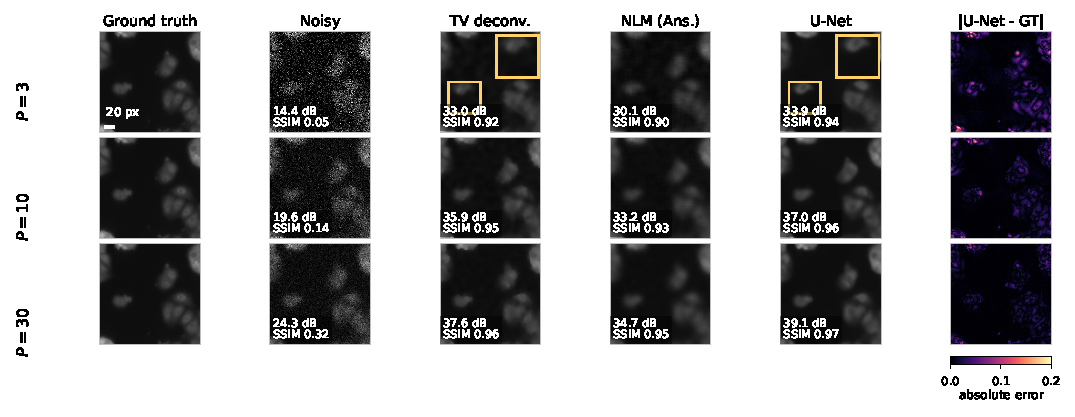
\includegraphics[width=\linewidth]{fig1_qualitative.pdf}
\caption{Qualitative reconstruction at $P=3,10,30$ on a
fixed $192\times192$ test crop (seed 7, not selected by performance). Columns:
ground truth, noisy input, TV deconvolution, NLM, mixed-dose U-Net, and the
absolute U-Net error. Scale bars are 20 pixels; the public BBBC014 release does
not include a pixel-size calibration, so physical units are not claimed. The
yellow boxes and insets magnify the same $60\times60$ region of the TV and
U-Net panels at $P=3$ (approximately 1.3$\times$). Panel PSNR values refer to this single
crop, not to the FOV means in Table~\ref{tab:perf}; all panels use the same
normalized intensity scale $[0,1]$. The network recovers boundaries and
internal texture that TV deconvolution smooths, and the error is concentrated
on edges.}
\label{fig:quant}
\end{figure}

TV deconvolution is the strongest classical method at every dose; TV denoising
without deblurring is
\DenGainThree\,dB below the network at $P=3$, whereas fair TV deconvolution
is \DecGainThree\,dB below. The gain is \DecGainThree, \DecGainThirty, and
\DecGainThreeHundred\,dB at 3, 30, and 300 against TV deconvolution, with no
monotonic dose trend; it is largest at $P=100$ ($1.45$\,dB) and smallest at
$P=3$ ($0.93$\,dB).

\subsection{Dose to matched quality}
Figure~\ref{fig:dose}a--c shows PSNR, SSIM, and foreground PSNR as a function
of dose. Fig.~\ref{fig:dose}e converts these curves into a fixed protocol:
choose the smallest dose that reaches 90\% success on the 20 validation FOVs,
then apply it unchanged to the test FOVs. The network needs a $3\times$ lower
dose $P$ (equivalently, a $3\times$ smaller photon budget) at PSNR 32\,dB and
SSIM 0.90, and $3.3\times$ lower at PSNR 34\,dB and foreground PSNR 26\,dB;
SSIM 0.85, SSIM 0.92, and foreground PSNR 24\,dB are ties. At PSNR 30\,dB the validation-selected U-Net dose reaches 80\% on test,
and at foreground PSNR 22\,dB the TV dose reaches 80\%, so neither factor is
claimed (SI S2b). Selecting the dose on the test FOVs gives an upper bound of
3--3.3$\times$ at five targets and four ties (SI S2b). The factors are
discrete and the 20-FOV sample is small; per-target CIs from the test-oracle
bootstrap are reported in SI S2b, where 96.6\% of resamples give at least
$3\times$ at PSNR 32\,dB.
The model is also not restricted to the five training doses: at $P=5,50,200$,
none of which was used in training, it reaches \HeldoutPFive, \HeldoutPFifty,
and \HeldoutPTwoHundred\,dB, within 0.02\,dB of log-dose interpolation between
the neighboring trained doses (SI S4c).

\begin{figure}[H]
\centering
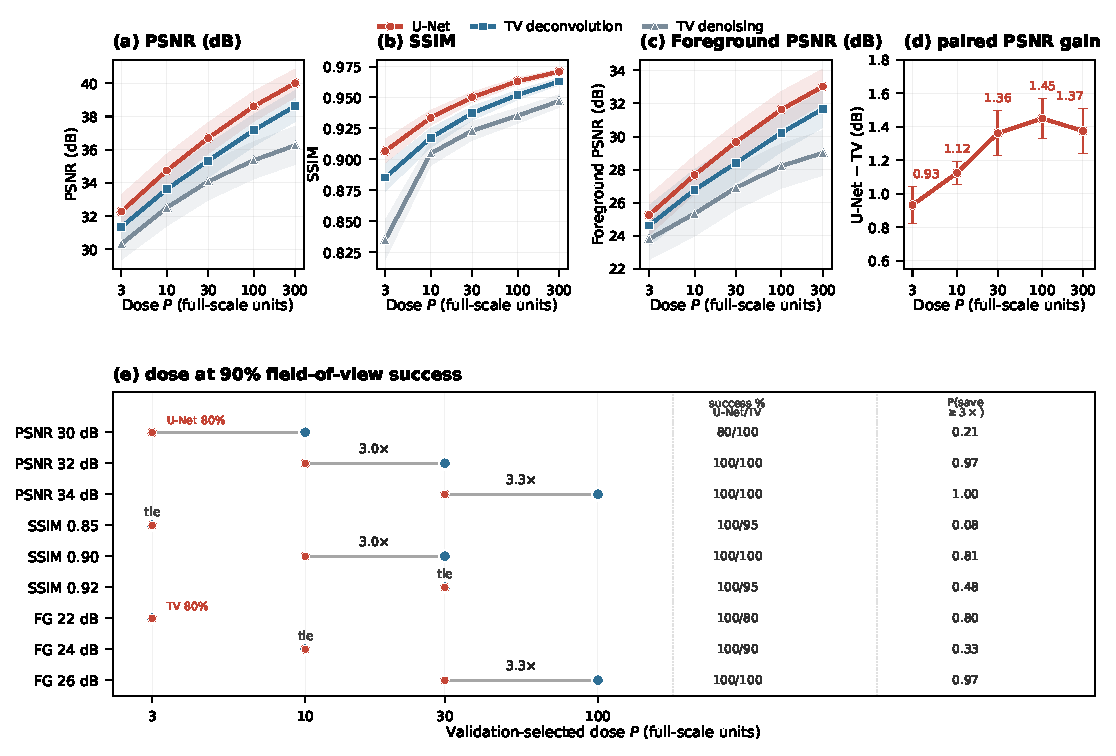
\includegraphics[width=\linewidth]{fig2_dose_response.pdf}
\caption{(a--c) PSNR, SSIM, and foreground PSNR versus dose $P$ on 20 held-out
FOVs; shaded bands are 95\% confidence intervals over FOVs. (d) Paired PSNR
gain of the U-Net over TV deconvolution on the same FOVs; error bars are 95\%
confidence intervals. (e) Validation-selected dose for 90\% success on
validation FOVs; blue dots are TV deconvolution and red dots the U-Net.
Factors are shown only when both methods also meet the 90\% criterion on
held-out FOVs; ``tie'' marks equal doses, and labels mark the method whose
validation-selected dose reaches only 80\% on test. Right-hand text columns
give the held-out success rate (U-Net/TV, \%) and the FOV-bootstrap probability
that the saving is at least $3\times$. Test-oracle doses and FOV-bootstrap CIs
are in SI S2b.}
\label{fig:dose}
\end{figure}



We also compared the mixed-dose model with a dose-conditioned variant and with
per-dose specialists. The budget-matched conditioned variant (64 channels, 48k
patches, 150 epochs) reaches \CondStrongPthree, \CondStrongPthirty, and
\CondStrongPonehundred\,dB at $P=3,30,100$, compared with
\BlindPthree, \BlindPthirty, and \BlindPonehundred\,dB for the blind model; it
is within \CondStrongDelta\,dB (\CondStrongLow--\CondStrongHigh\,dB) but
requires the photon count at inference. Per-dose specialists trained with the
same 64-channel/48k/150 budget reach \SpecPthree, \SpecPthirty, and
\SpecPonehundred\,dB at their own doses, within 0.1\,dB of the blind model, but
require one model per dose and the dose label. The blind model is therefore
preferred: it is within 0.05\,dB of the conditioned variant and within 0.1\,dB
of the specialists, with no acquisition metadata.

\subsection{Transfer across cell types and stains}
The model trained on BBBC014 channel~1 transfers without retraining to three
held-out datasets with different morphology and staining (Fig.~\ref{fig:cross}a,
Table~\ref{tab:cross}). At $P=30$ it gains \CrossDecFifteen\,dB over tuned
TV deconvolution on BBBC015, \CrossDecSixteen\,dB on BBBC016, and
\CrossDecEighteen\,dB on BBBC018; the in-domain gain is \CrossDecFourteen\,dB.
The external confidence intervals exclude zero, but the gains are smaller than
in-domain and the BBBC018 gain is modest; transfer helps but does not replace
in-domain training.

\begin{figure}[H]
\centering
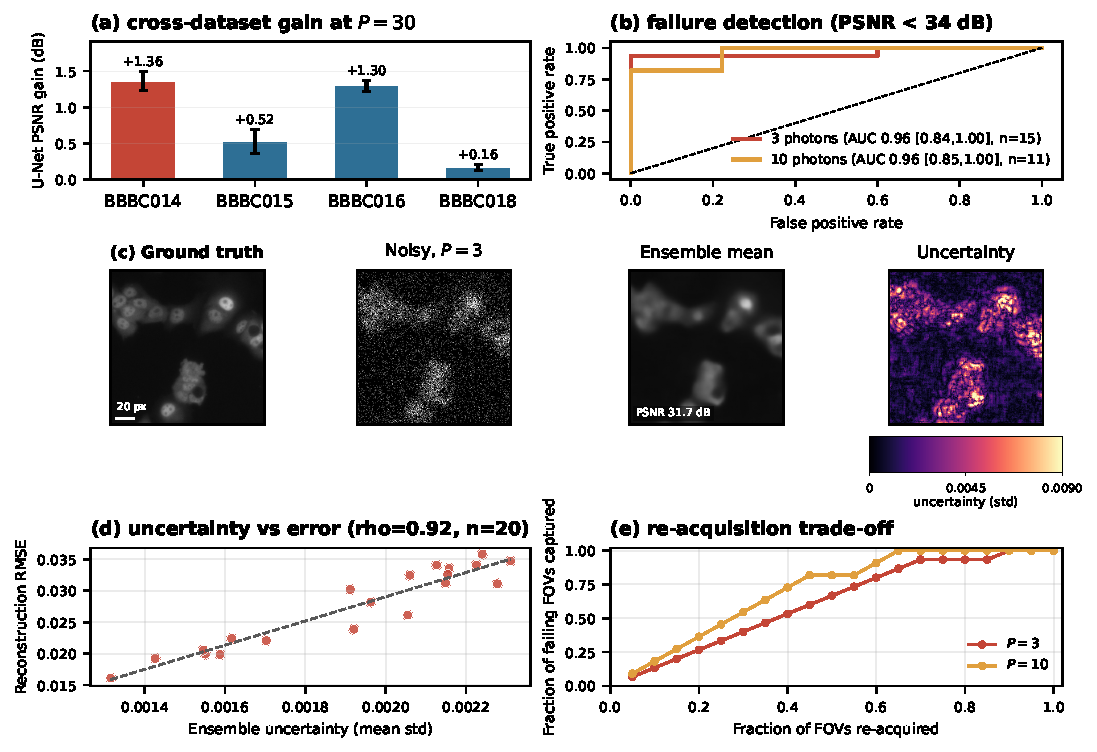
\includegraphics[width=\linewidth]{fig3_cross_uncertainty.pdf}
\caption{(a) Mean PSNR gain of the mixed-dose network over tuned TV
deconvolution at $P=30$ on four datasets; red is the in-domain dataset and
blue the external datasets; whiskers are 95\% bootstrap CIs. The external TV
weights are tuned on five separate fields per dataset. (b)
Failure-detection ROC from a base-budget uncertainty ensemble. (c) Example at
$P=3$ on a validation FOV: ground truth, noisy input, ensemble mean, and
uncertainty (standard deviation). (d) Uncertainty versus RMSE on held-out FOVs,
with a linear fit. (e) Re-acquisition trade-off: fraction of failing FOVs
captured versus fraction of FOVs re-acquired, at $P=3$ and 10. AUCs and 95\%
bootstrap CIs are in (b); at 30 only one FOV fails, so no AUC is shown.}
\label{fig:cross}
\end{figure}

\subsection{Uncertainty identifies unreliable fields}
The three-model ensemble provides a per-pixel uncertainty map
(Fig.~\ref{fig:cross}c). At $P=3$ the uncertainty is concentrated on
cell boundaries and on dim structures, where the error is largest. Across FOVs,
uncertainty correlates with reconstruction RMSE (Spearman $\rho=\RhoThree$), and
it separates FOVs that fail a 34\,dB target from those that succeed with AUC
\AucThree\ (95\% CI 0.84--1.00) at $P=3$ and \AucTen\ (0.85--1.00) at 10
(Fig.~\ref{fig:cross}b,e; SI S4). At 30 only
\NFailThirty\ of 20 FOVs fell below the target, so no AUC is reported. This provides a practical quality-control signal: fields with high
uncertainty can be re-acquired or interpreted conservatively without a
ground-truth image.



\begin{table}[t]
\centering
\caption{Cross-dataset PSNR at $P=30$. BBBC014 uses its 20 test
FOVs; each external dataset is split into five validation fields for TV tuning
and 15 held-out fields for evaluation. The model is trained only on BBBC014
channel~1 and external evaluation is zero-shot; TV deconvolution is tuned per
dataset on its five validation fields.}
\label{tab:cross}
\begin{tabular}{lccc}
\toprule
Dataset & TV deconv & U-Net & $\Delta$ [95\% CI] \\
\midrule
BBBC014 (20 test FOVs) & 35.34 & 36.70 & +1.36 [+1.23, +1.49] \\
BBBC015 (15 fields) & 34.63 & 35.15 & +0.52 [+0.35, +0.68] \\
BBBC016 (15 fields) & 33.81 & 35.10 & +1.30 [+1.22, +1.37] \\
BBBC018 (15 fields) & 25.62 & 25.78 & +0.16 [+0.12, +0.21] \\
\bottomrule
\end{tabular}

\end{table}

\subsection{Real noisy/clean pairs}
To test whether the restoration gain survives real noise, we trained the same
U-Net topology (48 channels) on 1{,}951 real noisy/clean pairs from the
AI4Life-MDC25 release
and evaluated it on \RealN\ held-out pairs from the same source
(Fig.~\ref{fig:real}, Table~\ref{tab:real}). The network reaches
\RealUnetP\,dB PSNR and \RealUnetS\ SSIM, compared with \RealBMThreeP\,dB and
\RealBMThreeS\ for affine-calibrated tuned BM3D, \RealNlmP\,dB and \RealNlmS\ for NLM, and
\RealNoisyP\,dB for the noisy input. BM3D and NLM are within 0.05\,dB of each
other; the paired gain is \RealGain\,dB over BM3D (95\% CI \RealCI; exact
Wilcoxon $p=\RealPvalue$), \RealGainNlm\,dB over NLM, and \RealGainTv\,dB over
TV denoising; the network wins on \RealWins\ of \RealN\ pairs. A budget-matched
DnCNN (16k patches, 80 epochs) reaches \RealDncnnP\,dB and \RealDncnnS\ SSIM,
\RealDncnnGain\,dB above affine-calibrated BM3D and only
\RealUnetGainDncnn\,dB below the U-Net (95\% CI \RealUnetDncnnCI;
\RealUnetDncnnWins\ of 243 pairs). The gain over classical methods is therefore
shared by a second deep architecture, while the U-Net retains a small edge. This is an
in-source real-noise result: training and test pairs come from the same
acquisition protocol, with disjoint fields and no near-duplicate images. The
real pairs contain no blur component, so they validate denoising within a
matched protocol, not deblurring.

The FMD release was evaluated on a pre-specified stratified subset of 150 of
its 301 held-out fields (SI S7b). With per-microscope-tuned baselines, the
U-Net reaches \FmdUnetP\,dB and \FmdUnetS\ SSIM versus \FmdBMThreeP\,dB and
\FmdBMThreeS\ for BM3D (+\FmdGain\,dB, \FmdWins/\FmdN; SI S7b). These numbers
are not affine-calibrated, so FMD remains a secondary upper-bound check and is
not used as a headline; the main real-data evidence is the nuclei set above.

When the same trained model is applied to the 20 large BBBC006 fields in the
same release, the ranking reverses: the network reaches \LargeRealUnetP\,dB,
below the raw classical baselines BM3D (\LargeRealBMThreeP\,dB), NLM
(\LargeRealNlmP\,dB), and TV (\LargeRealTvP\,dB). The large
fields have 16-bit saturated references and a different noise model, so this is
a cross-source transfer failure rather than a contradiction of the in-source
result. It confirms that matching the training and deployment acquisition
remains necessary, and it is the main reason we describe the dose sweep as a
controlled simulation rather than a real low-dose validation.

\begin{table}[t]
\centering
\caption{Real noisy/clean pairs from AI4Life-MDC25 (Jacquemet source).
\RealN\ held-out nuclei fields; classical parameters are tuned and
affine-calibrated on validation fields; DnCNN is a second supervised deep
baseline. PSNR in dB.}
\label{tab:real}
\begin{tabular}{lcc}
\toprule
Method & PSNR (dB) & SSIM \\
\midrule
\multicolumn{3}{l}{\emph{AI4Life nuclei, \RealN\ held-out fields}} \\
Noisy input & \RealNoisyP & \RealNoisyS \\
TV denoising & \RealTvP & \RealTvS \\
NLM & \RealNlmP & \RealNlmS \\
BM3D & \RealBMThreeP & \RealBMThreeS \\
DnCNN (supervised) & \RealDncnnP & \RealDncnnS \\
U-Net & \RealUnetP & \RealUnetS \\
\bottomrule
\end{tabular}

\end{table}

\begin{figure}[H]
\centering
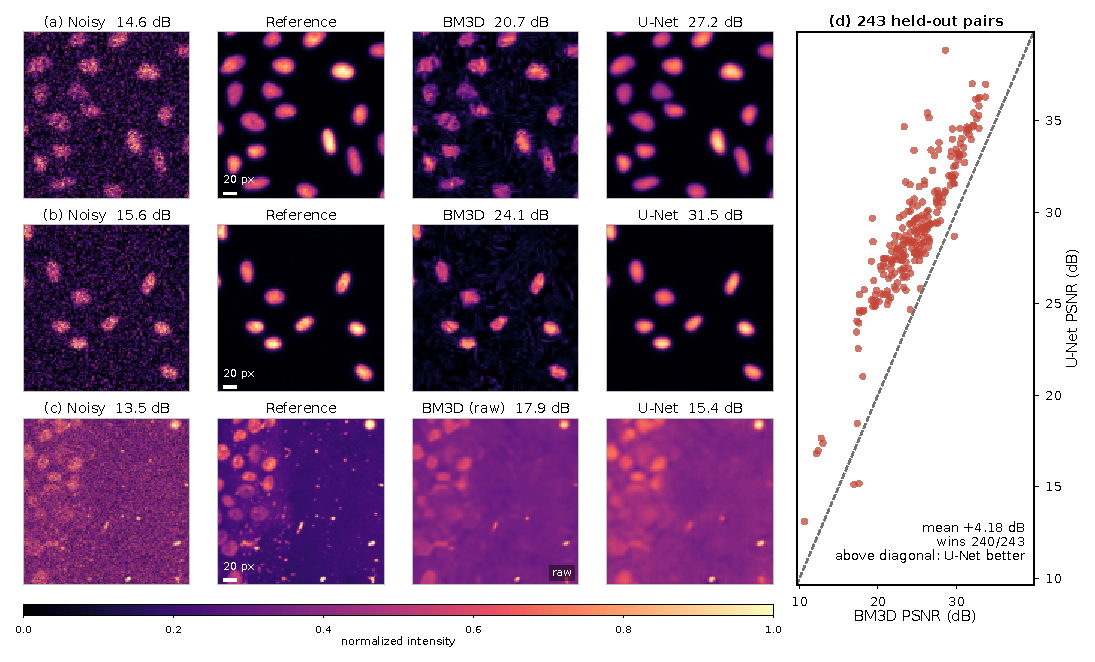
\includegraphics[width=\linewidth]{fig4_real.pdf}
\caption{Real-data validation on held-out AI4Life-MDC25 pairs. (a,b) Two
fixed held-out pairs at the 25th and 75th percentile of U-Net PSNR (median-quality
examples, not cherry-picked best cases), showing the noisy input, clean reference,
affine-calibrated BM3D, and U-Net; numbers are per-pair PSNR. (c) A large
BBBC006 field from the same release (fixed field and crop), where the same
weights fail under cross-source transfer; BM3D is raw here. (d) Per-pair PSNR
of the U-Net versus BM3D for \RealN\ held-out pairs; the dashed line is $y=x$,
and \RealWins\ of \RealN\ pairs lie above it. All image panels use one shared
normalized intensity scale $[0,1]$, shown by the single colorbar; scale bars are
20 pixels. The BM3D panel in (c) is raw and uncalibrated, as tagged in the
panel.}
\label{fig:real}
\end{figure}

\subsection{Controls, PSF robustness, and speed}
A phase-scrambled control with the same 64-channel/48k/150 budget, trained on
surrogates with the same power spectrum but no spatial structure, reaches
\ScrPthree, \ScrPthirty, and \ScrPonehundred\,dB at $P=3,30,100$,
below both the real model (\UNetPthree, \UNetPthirty, and \UNetPonehundred\,dB)
and TV deconvolution (\DecPthree, \DecPthirty, and \DecPonehundred\,dB;
Supplementary Information). The gain over the classical
baseline therefore requires learned sample structure, not just extra denoising
capacity.

The mixed-dose model tolerates a modest Gaussian-width mismatch: at $P=30$ it reaches
\SigmaUPfifteen, \SigmaUPtwo, and \SigmaUPtwopfive\,dB for $\sigma=1.5,2.0,2.5$,
compared with \SigmaDecfifteen, \SigmaDectwo, and \SigmaDectwopfive\,dB for
TV deconvolution with $\lambda$ retuned at each width (0.04 selected in all
three cases; Supplementary Information); the network is ahead by 1.07, 1.36,
and 1.00\,dB at the three widths. The
Gaussian-trained model does not transfer to a PSF with a different shape and
width: with an in-focus Airy PSF (NA 1.4, 520\,nm, 100\,nm pixels; FWHM about
1.9 pixels, narrower than the $\sigma=2$ training kernel), it reaches
\AiryStrongUThree,
\AiryStrongUThirty, and \AiryStrongUThreeHundred\,dB at $P=3/30/300$, i.e.
\AiryStrongGainThree, \AiryStrongGainThirty, and
\AiryStrongGainThreeHundred\,dB versus TV deconvolution with the correct PSF. A
model trained on a 50/50 Gaussian/Airy mixture recovers the high-dose
performance: \AiryUThree, \AiryUThirty, and \AiryUThreeHundred\,dB (gains
\AiryGainThree, \AiryGainThirty, and \AiryGainThreeHundred\,dB; 95\% CIs
\AiryCIThree, \AiryCIThirty, and \AiryCIThreeHundred; 20/20 FOVs), while
retaining \PsfMixGaussPThree, \PsfMixGaussPThirty, and
\PsfMixGaussPThreeHundred\,dB on the Gaussian benchmark. The dose-agnostic
result is therefore not tied to the exact Gaussian kernel, provided the
training distribution covers the deployed PSF. An
exploratory dose+PSF-conditioned model (32 channels, 20k patches, 60 epochs;
it receives both the dose $P$ and $\sigma$) reached 36.69, 36.03, and
35.44\,dB at the same $\sigma$ values, 0.23--0.67\,dB below the strong blind
model; because it is neither budget-matched nor blind, we do not adopt it
(\texttt{results/dscond\_eval.json}). Adding Gaussian read
noise of 0.005 or 0.01 (1.3 or 2.6 8-bit counts) at $P=30$ changed the
network and fair TV values by at most 0.04\,dB (SI).

Inference takes \SpeedGPU\,ms per $128\times128$ patch on an A100 and
\SpeedCPU\,ms on one CPU core, versus \SpeedTV\,ms for 30-iteration ADMM TV
deconvolution on one CPU core. The network is therefore \SpeedFactorCPU$\times$
faster on the same CPU core and \SpeedFactorGPU$\times$ faster when the network
runs on the GPU. A full $1360\times1024$ FOV requires about 85 patches, i.e.,
about 0.1\,s on the GPU or 2.5\,s on one CPU core: this supports interactive and
many online workflows, but not full-FOV frame-rate feedback on a single CPU
core.





\subsection{Adaptive allocation is target-dependent}
We also tested whether a cheap preview and per-FOV uncertainty could choose a
different dose for each field. An oracle with access to each FOV's full
dose-response would save 42--71\% of photons across the tested targets, but a ground-truth-free policy
calibrated on validation FOVs did not consistently beat the best fixed dose at
matched test success; details are in the Supplementary Information. We
therefore recommend the fixed protocol dose read from Fig.~\ref{fig:dose}e
rather than per-FOV allocation.

\section{Discussion}
The gain has two sources. Denoising capacity accounts for part of it, but the
phase-scrambled control shows that capacity alone does not beat fair TV
deconvolution. The rest comes from a learned prior over sample structure: at
$P=3$ the input retains little more than the
position and approximate shape of a cell, yet the network recovers boundaries
and internal texture that TV deconvolution smooths away. The same prior raises
the achievable quality at high dose, where the classical method saturates. The
dose-conditioned and specialist comparisons show that this prior can be learned
from mixed doses without a dose input; the photon count is not needed at
inference. Consistent with this, a linear probe on simple image statistics
identifies the five dose levels with 97.9\% accuracy (100\% with a small CNN;
SI S8), so the information needed to adapt the effective regularization is
present in the noisy input.

With validation-selected doses the protocol yields a 3--3.3$\times$ lower
photon budget at four targets and ties at three; two validation selections miss
the held-out criterion, and the test-oracle upper bound is five savings and
four ties. At SSIM 0.85 the classical method is already at the same dose, so there
the network's advantage is the quality ceiling rather than the threshold. The
cross-dataset
gains suggest that the prior is not tied to one cell type or stain, although
they are smaller outside the training distribution.

\paragraph{Simulation.}
The noise is simulated as Gaussian-blurred Poisson noise with a known,
spatially invariant PSF; camera read noise, background structure, and optical
aberrations are absent. The high-SNR reference is itself diffraction-limited,
so the network removes an additional synthetic Gaussian blur rather than the
microscope PSF; the experiment tests photon efficiency under controlled blur,
not a full optical reconstruction of an unknown object. The PSF tests cover
Gaussian widths of 1.5--2.5 pixels and an in-focus Airy PSF; a PSF-mixed model
retains the gain under Airy, but arbitrary, aberrated, or depth-varying PSFs
remain untested. The simulation model is trained on one dataset and evaluated
zero-shot on three others; the external gains are smaller, and training on a
mixture may improve them.

\paragraph{Real data.}
A downstream BBBC039 nuclei-mask check with per-dose tuned TV found only a
small Dice gain (0.795 versus 0.773 at $P=1$; SI), so the restoration advantage
does not automatically translate into a large segmentation gain. The real-data
check is in-source: on \RealN\ held-out AI4Life pairs the real-data model beats
tuned BM3D by \RealGain\,dB, but the same weights fail on the large BBBC006
fields in the same release, which differ in bit depth, saturation, and noise
model. Real paired data therefore support restoration within a matched
acquisition protocol, not the cross-source dose claim. A label-free
J-invariant variant \cite{batson2019noise2self} trained only on the noisy
images reached 17.89\,dB on the held-out set,
below tuned BM3D (21.30\,dB, uncalibrated), so the paired clean references are necessary for
the present gain. The FMD check uses a pre-specified 150-field subset and
requires retraining on FMD; it is not a zero-shot transfer, and the remaining
151 test fields were not evaluated.

\paragraph{Uncertainty and hallucination.}
The uncertainty ensemble uses the conditioned variant; because conditioning
changes accuracy only marginally, we expect the calibration to transfer, but
this is not tested directly. Learned restoration can produce plausible but incorrect structure \cite{blau2018perception}; uncertainty
flags unreliable fields but does not prove that a confident reconstruction is
artifact-free. Validation on matched real low-dose data remains necessary
before quantitative biological use.

The closest prior work differs in mechanism and evidence. FFDNet conditions a
denoising network on a noise level, and CARE learns a supervised restoration
mapping from paired images. Here a single mixed-dose model needs neither a
noise-level input nor per-dose retraining, and it is within 0.05\,dB of the
conditioned variant. Ye et al. \cite{ye2025uncertainty} use uncertainty to
drive adaptive rescanning; our protocol is a fixed widefield acquisition, and
an adaptive extension is reported as a negative result in the SI. Liu et al.
\cite{liu2020degeneration} use a model-based deep prior, whereas our network is
trained end-to-end across dose. Qiao et al. \cite{qiao2024zsdeconvnet} remove
the need for paired clean targets by zero-shot learning from noisy images; that
addresses the supervision axis, whereas the matched-success protocol here
addresses the dose axis and measures the photon-budget gain against a
per-dose-tuned classical baseline. Sheneman et al. \cite{sheneman2025nearzero}
demonstrate a hardware near-zero-photon microscope, whereas this is a
controlled simulation
of the dose sweep with an in-source real-data check.

Operationally, a laboratory would train once over the dose range of interest,
read a fixed dose from the protocol curve for the desired success rate, and use
ensemble uncertainty to flag fields that need more light. The approach requires no change to the
microscope and no photon-count metadata at inference; the simulation model is
trained once across the dose range, and the real-data model is trained once on
paired images from the deployment protocol. Its speed is compatible with online
processing budgets.

\section*{Conclusions}
One mixed-dose U-Net, with no photon-count input, matches or beats a fully
tuned TV-ADMM baseline across a 100-fold dose range and, at matched success,
uses a threefold lower photon budget. On real paired data it improves over
affine-calibrated BM3D by more than 4\,dB and wins on all but three fields. The
gain is not a capacity effect: conditioning on dose adds less than
\CondStrongDelta\,dB, and a budget-matched phase-scrambled control remains below
TV. For a fixed acquisition protocol, these results argue that dose metadata
and per-dose retuning are not required, and that restoration methods should be
compared by the photon budget needed at a matched success rate. The next step
is prospective validation on real low-dose acquisitions and other microscope
PSFs.

\section*{Data and code availability}
All datasets are public: BBBC014, BBBC015, BBBC016, BBBC018, and BBBC039 from
the Broad Bioimage Benchmark Collection \cite{ljosa2012bbbc}, AI4Life-MDC25-Nuclei
\cite{ai4life_mdc25_2025} (Zenodo 15624741, CC~BY~4.0), and AI4Life-MDC25-FMD
\cite{ai4life_mdc25_fmd_2025} (Zenodo 15761900, CC~BY~4.0), with accession
numbers and licenses listed in the Methods. Code for data splits, training, baselines,
statistics, and figures, together with the JSON result files and checkpoints,
will be released with the manuscript.

\begingroup
\small
\bibliographystyle{unsrt}
\bibliography{references}
\endgroup
\end{document}
